\documentclass{article}

\usepackage{microtype}
\usepackage{graphicx}
\usepackage{booktabs}
\usepackage{hyperref}

\newcommand{\theHalgorithm}{\arabic{algorithm}}

\usepackage[preprint]{icml2026}

\usepackage{amsmath}
\usepackage{amssymb}

\icmltitlerunning{IsoColBERT: Token-Level Isotropy for Multilingual Late Interaction}

\begin{document}

\twocolumn[
  \icmltitle{IsoColBERT: Token-Level Isotropy Regularization for\\
    Multilingual Late-Interaction Retrieval}

  \icmlsetsymbol{equal}{*}

  \begin{icmlauthorlist}
    \icmlauthor{Minh Tran}{harvard}
    \icmlauthor{Isaac Chang}{harvard}
    \icmlauthor{Ingrid Chien}{harvard}
  \end{icmlauthorlist}

  \icmlaffiliation{harvard}{Harvard University}

  \icmlcorrespondingauthor{Minh Tran}{minhtran@college.harvard.edu}

  \icmlkeywords{multilingual retrieval, late interaction, ColBERT, isotropy, contrastive learning}

  \vskip 0.3in
]

\printAffiliationsAndNotice{}

\begin{abstract}
Late-interaction multilingual retrievers such as ColBERT score query-document pairs at the token level via MaxSim, placing the geometry of individual token vectors at the center of retrieval quality. We show that multilingual ColBERT trained with bitext InfoNCE produces token vectors that are anisotropic: they concentrate in a narrow cone with effective rank well below the embedding dimension, with the target-side language collapsing harder than the source-side. To address this, we introduce \textbf{IsoColBERT}, a single regularizer term added to the InfoNCE training objective that penalizes the mean squared off-diagonal cosine similarity of valid token vectors in each batch, with zero cost at inference. Across three random seeds on FLORES+, IsoColBERT improves MaxSim P@1 by $3.45$ percentage points on English-Swahili (every seed individually positive) and $1.99$ percentage points on English-Arabic, with the gain extending zero-shot to two further low-resource languages (Nepali $+1.46$ pp, Tamil $+0.88$ pp), while leaving high-resource pairs unchanged. Mechanism ablations rule out localized and matching-level placements as substitutes for full-manifold regularization. The gains concentrate where pretrained signal is weakest, suggesting that token geometry is a tractable lever for low-resource multilingual retrieval.
\end{abstract}

\section{Introduction}
\label{sec:intro}

Cross-lingual search and retrieval-augmented generation depend on multilingual dense retrievers that match English queries to documents in dozens of target languages. Late-interaction retrievers, introduced by ColBERT \citep{khattab2020colbert} and refined by ColBERTv2 \citep{santhanam2022colbertv2}, differ from single-vector encoders in a fundamental way: they score each (query, document) pair at the level of individual token vectors via a MaxSim operation. Every query token finds its best matching document token, and the per-token best matches are summed. Recent multilingual extensions such as ColBERT-XM \citep{louis2024colbertxm} and Jina-ColBERT-v2 \citep{jha2024jinacolbert} extend late interaction to multiple languages, alongside dense single-vector retrievers like LaBSE \citep{feng2022labse}, Contriever \citep{izacard2022contriever}, and multilingual E5 \citep{wang2024me5}.

Token-level scoring places token geometry at the center of retrieval quality. Contextual embeddings from pretrained language models are known to be anisotropic: representations of unrelated tokens concentrate in a narrow cone of the hypersphere, with mean pairwise cosine similarity well above zero \citep{ethayarajh2019contextual,mu2018allbutthetop,gao2019representation}. In single-vector retrievers, this anisotropy is partially masked: the score depends on a sentence-pooled representation, so token-level concentration is averaged out before the comparison. In late-interaction retrievers, every token participates in the score through a hard argmax. If many candidate tokens have similar cosine similarity to a query token, the argmax becomes unstable and the score depends weakly on the identity of the true match. We expect the pathology to be most damaging on low-resource cross-lingual pairs, where multilingual encoders inherit the weakest pretrained signal and the retrieval headroom is largest. \citet{rajaee2022isotropy} document anisotropy in multilingual BERT but stop short of evaluating its consequences for retrieval.

Existing remedies for anisotropy are designed for single-vector encoders and either operate post-hoc or pool away token-level structure. BERT-flow \citep{li2020sentenceembeddings} maps sentence embeddings to an isotropic Gaussian with a learned normalizing flow. WhiteningBERT \citep{huang2021whiteningbert} applies a closed-form whitening transform. SimCSE \citep{gao2021simcse} induces partial isotropy as a side effect of dropout-based contrastive learning. Two recent papers extend isotropy mitigation to ColBERT, both in monolingual settings: \citet{jung2023isotropic} apply post-hoc whitening to ColBERT token vectors on English retrieval benchmarks, and \citet{kim2024hil} propose a hybrid isotropy/anisotropy architecture for English zero-shot transfer. The most relevant training-time regularizer, I-STAR \citep{rudman2024istar}, adds a differentiable isotropy penalty to fine-tuning for classification and concludes that \emph{decreasing} isotropy can help. The question of whether a training-time, token-level regularizer can improve multilingual late-interaction retrieval, and whether the direction of the effect agrees with single-vector or contradicts it, remains open.

This paper presents IsoColBERT, a single-term regularizer added to the InfoNCE training objective of multilingual ColBERT. The regularizer penalizes the mean squared off-diagonal cosine similarity of the valid token vectors in each training batch, with one hyperparameter for its weight and zero cost at inference time. Across three random seeds on FLORES+, IsoColBERT improves MaxSim P@1 by $3.45$ percentage points on English-Swahili (every seed individually positive) and by $1.99$ percentage points on English-Arabic, with the gain extending zero-shot to two further low-resource languages (Nepali $+1.46$ pp, Tamil $+0.88$ pp), while leaving high-resource pairs (EN-ES, EN-FR, EN-DE) unchanged. Token-level geometry shifts as designed: intra-cosine drops and effective rank rises, with the largest shift on Spanish tokens, which collapse hardest under bitext contrastive pressure. Mechanism ablations against two alternative placements rule out localized and matching-level regularization as substitutes for the full-manifold objective.

This paper makes the following contributions.
\begin{enumerate}
    \item We identify token-level anisotropy as a measurable pathology in multilingual late-interaction retrieval. Vanilla ColBERT trained with bitext InfoNCE produces token vectors with intra-cosine of $0.29$ and effective rank of $102$ on Spanish tokens, well below the geometry of English tokens trained under the same objective.
    \item We introduce IsoColBERT, a one-term training-time regularizer that improves token geometry monotonically with its weight and recovers significant retrieval accuracy on low-resource language pairs. The method adds zero inference cost and requires no architectural changes.
    \item In contrast to prior work that attributes multilingual retrieval gaps to data scarcity or supervision, and in contrast to recent isotropy regularization results that find \emph{decreasing} isotropy helps classification fine-tuning, we show that for late-interaction retrieval the dominant correctable cause is geometric and the productive direction is toward higher isotropy across the full token manifold.
\end{enumerate}

\section{Related Work}
\label{sec:related}

\paragraph{Anisotropy in contextual embeddings.} \citet{ethayarajh2019contextual} document that BERT, ELMo, and GPT-2 produce contextual embeddings that occupy a narrow cone of the hypersphere at every layer, with the effect intensifying with depth. \citet{mu2018allbutthetop} show that subtracting the mean and removing top principal components (``all-but-the-top'') makes static word embeddings more isotropic and improves downstream tasks. \citet{gao2019representation} identify a parallel phenomenon in language generation models, where weight-tied softmax training pushes learned embeddings into a degenerate cone, and propose a cosine-based regularizer to widen it. For sentence-level encoders, BERT-flow \citep{li2020sentenceembeddings} learns an invertible flow to an isotropic Gaussian, and WhiteningBERT \citep{huang2021whiteningbert} applies a closed-form whitening transform at inference. \citet{rajaee2022isotropy} extend the diagnostic analysis to multilingual BERT and show that anisotropy is present across all languages, with substantial variation between high- and low-resource languages. These works diagnose and mitigate anisotropy at the sentence level using post-hoc or pooling-based fixes. We study token-level geometry in late-interaction retrieval, where pooling does not occur and the regularizer must operate at training time.

\paragraph{Contrastive learning and uniformity.} \citet{wang2020understanding} decompose the asymptotic InfoNCE loss into an alignment term and a uniformity term and show that directly optimizing both recovers contrastive training. Uniformity on the hypersphere is closely related to isotropy: a uniformly distributed set of $L_2$-normalized vectors has zero mean pairwise cosine similarity. SimCSE \citep{gao2021simcse} relies on this connection implicitly, using dropout as data augmentation to induce both alignment and uniformity for sentence embeddings. \citet{xiao2023isotropy} analyze how contrastive losses partially induce isotropy in sentence encoders. Our regularizer is a token-level analog of the Wang and Isola uniformity term, applied inside sequence models where InfoNCE operates at the sentence level but the score function operates at the token level.

\paragraph{Late-interaction retrieval.} ColBERT \citep{khattab2020colbert} introduces late interaction with token-level MaxSim scoring. ColBERTv2 \citep{santhanam2022colbertv2} improves quality and efficiency through denoised supervision and residual compression of token vectors. PLAID \citep{santhanam2022plaid} provides an efficient retrieval engine for compressed ColBERTv2 indexes. Recent multilingual extensions include ColBERT-XM \citep{louis2024colbertxm} and Jina-ColBERT-v2 \citep{jha2024jinacolbert}, both of which scale late interaction to many languages through modular architectures and additional training data. These works improve quality through better training data, supervision, or compression. We improve quality through a geometric prior on the token vectors themselves.

\paragraph{Multilingual dense retrieval.} XLM-R \citep{conneau2020xlmr} is the dominant multilingual backbone for dense retrievers. LaBSE \citep{feng2022labse} combines masked and translation language modeling with margin-based contrastive learning for cross-lingual sentence embeddings. Contriever \citep{izacard2022contriever} introduces unsupervised contrastive pre-training for dense retrieval and extends it to multiple languages. Multilingual E5 \citep{wang2024me5} uses large-scale weakly supervised contrastive pre-training followed by supervised fine-tuning. The standard multilingual retrieval benchmarks include MIRACL \citep{zhang2023miracl} for monolingual ad-hoc retrieval across 18 languages and mMARCO \citep{bonifacio2021mmarco} for multilingual passage ranking. These efforts focus on data and supervision; we hold both fixed and intervene only on training-time geometry.

\paragraph{Isotropy regularization for retrieval and beyond.} The closest prior work to ours applies isotropy techniques to ColBERT or to training-time regularization. \citet{jung2023isotropic} apply post-hoc normalizing flow and whitening to ColBERT and RepBERT, both sentence-level and token-level, on English retrieval benchmarks. \citet{kim2024hil} propose a hybrid isotropy/anisotropy ColBERT architecture for zero-shot transfer on BEIR. Both are monolingual and do not target the cross-lingual regime where pretrained signal asymmetry is the dominant source of geometric collapse. I-STAR \citep{rudman2024istar} adds a differentiable isotropy regularizer to fine-tuning and reports that \emph{decreasing} isotropy can help classification tasks, suggesting that the productive direction is task-dependent. In a separate line, \citet{ji2023isotropic} apply isotropy interventions to zero-shot cross-lingual transfer on classification, not retrieval. Our paper occupies a different point in this design space: training-time, token-level, multilingual, late-interaction, low-resource. We address the I-STAR result directly: for MaxSim retrieval, the productive direction is toward higher isotropy across the full token manifold.

\section{Method}
\label{sec:method}

\subsection{Background: ColBERT and MaxSim Retrieval}
\label{sec:method-background}

Late-interaction retrieval, introduced by ColBERT \citep{khattab2020colbert}, scores query-document pairs at the level of individual token vectors. Given a query $Q$ and document $D$, an encoder $E_\theta$ produces sequences of token vectors $\{q_i\}_{i=1}^{|Q|}$ and $\{d_j\}_{j=1}^{|D|}$, each projected to dimension $k$ and $L_2$-normalized. The relevance score is the sum over query tokens of the best matching cosine similarity in the document:
\begin{equation}
\label{eq:maxsim}
\mathrm{score}(Q, D) = \sum_{i=1}^{|Q|} \max_{1 \le j \le |D|} \langle q_i, d_j \rangle.
\end{equation}
We follow the standard cross-lingual ColBERT setup: an XLM-RoBERTa encoder with a 128-dimensional linear projection \citep{conneau2020xlmr}. The model is trained with symmetric in-batch InfoNCE \citep{gao2021simcse,wang2020understanding} over aligned source-target pairs:
\begin{equation}
\label{eq:infonce}
\mathcal{L}_{\mathrm{InfoNCE}} = \tfrac{1}{2}\bigl[ \ell(S, T) + \ell(T, S) \bigr],
\end{equation}
where $\ell(S, T)$ is the cross-entropy of the temperature-scaled scores from \eqref{eq:maxsim} against the diagonal positive assignment. Concretely, we compute a single $B \times B$ MaxSim score matrix with source tokens as queries and target tokens as documents, and apply symmetric cross-entropy along both axes by transposing this matrix; because \eqref{eq:maxsim} is asymmetric in its query and document arguments, this is not identical to recomputing MaxSim with target tokens as queries. We use the transposed form throughout — the same symmetric-cross-entropy pattern standard in CLIP-style contrastive pretraining.

\subsection{Token-Level Anisotropy}
\label{sec:method-anisotropy}

Anisotropy in single-vector encoders refers to the empirical observation that contextual embeddings concentrate in a narrow cone of the hypersphere, with mean cosine similarity between random vectors well above zero \citep{ethayarajh2019contextual,gao2019representation,mu2018allbutthetop}. For sentence-pooled representations, the consequences are partially masked: pooling averages over tokens and downstream similarity is computed once per pair. Late-interaction scoring is qualitatively different. Every query token participates in \eqref{eq:maxsim} through a hard argmax, so the score depends on the angular separation between many candidate token directions.

We quantify token-level anisotropy with two metrics computed on a fixed pool of valid (non-pad) token vectors $X \in \mathbb{R}^{N \times k}$:

\paragraph{Intra-cosine similarity.} The mean off-diagonal cosine similarity,
\begin{equation}
\label{eq:intracos}
\mathrm{IC}(X) = \frac{1}{N(N-1)} \sum_{i \ne j} \langle x_i, x_j \rangle.
\end{equation}
A value near zero indicates an isotropic spread; values close to one indicate collapse.

\paragraph{Effective rank.} The exponential entropy of the normalized singular value distribution \citep{wang2020understanding}: given singular values $\sigma_1, \ldots, \sigma_k$ of $X$ and probabilities $p_i = \sigma_i / \sum_j \sigma_j$,
\begin{equation}
\label{eq:erank}
\mathrm{eRank}(X) = \exp\!\Bigl( - \sum_{i=1}^{k} p_i \log p_i \Bigr).
\end{equation}
Effective rank counts the number of dimensions that the embedding space actively uses; collapse pulls it toward 1.

We will show in Section~\ref{sec:results} that token vectors of multilingual ColBERT trained with vanilla InfoNCE exhibit intra-cosine of $0.20$ on English tokens and $0.29$ on Spanish tokens, with effective rank below $106$ out of a possible $128$. The asymmetry is consistent with the geometry of bitext contrastive training: in an English-Spanish pair, the Spanish side carries most of the contrastive gradient pressure and so collapses harder.

\begin{figure}[t]
\centering
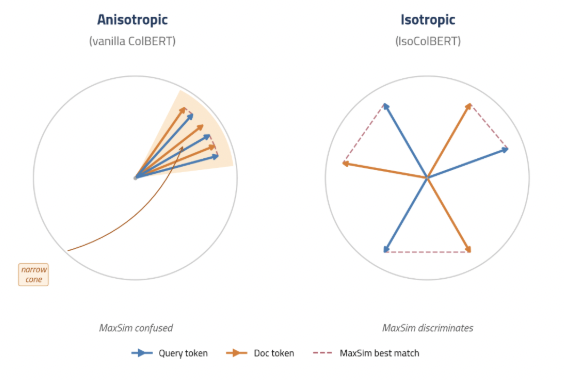
\includegraphics[width=0.95\columnwidth]{figs/fig_idea.png}
\caption{Effect of token-level anisotropy on MaxSim retrieval. Left: under vanilla training, token vectors concentrate in a narrow cone, so query tokens and document tokens have similar cosine similarity to many candidates and MaxSim cannot cleanly discriminate the true match. Right: under IsoColBERT, tokens spread across the hypersphere, giving MaxSim a larger margin between the true match and confusers.}
\label{fig:idea}
\end{figure}

\subsection{The IsoColBERT Objective}
\label{sec:method-iso}

If token-level anisotropy degrades MaxSim, the natural remedy is to add a training-time penalty that pushes token vectors apart. We define a per-batch isotropy regularizer that penalizes the squared off-diagonal cosine similarities of the valid token vectors in the batch:
\begin{equation}
\label{eq:reg}
R(X) = \frac{1}{N(N-1)} \sum_{i \ne j} \langle x_i, x_j \rangle^2.
\end{equation}
The squared form has two properties we want. It is non-negative, with its minimum attained when all pairs are orthogonal. We do not reach this minimum in practice: with $N \le 256$ token vectors subsampled into $k=128$ dimensions, at most $k$ pooled vectors can be mutually orthogonal, so the exact zero is unattainable in our setting. The loss nonetheless continues to drive pairwise cosine similarities toward zero, spreading the pooled vectors as far apart as the embedding dimension permits. The squared form also penalizes negative correlations as well as positive ones, which is appropriate on the hypersphere where $\langle x_i, x_j \rangle$ already takes values in $[-1, 1]$.

The full IsoColBERT objective adds \eqref{eq:reg} to the InfoNCE loss with weight $\lambda$, applied symmetrically to the query and document token banks:
\begin{equation}
\label{eq:loss}
\mathcal{L} = \mathcal{L}_{\mathrm{InfoNCE}} + \lambda \cdot \tfrac{1}{2}\bigl( R(X_Q) + R(X_D) \bigr).
\end{equation}
$X_Q$ and $X_D$ are the pooled valid token matrices for queries and documents in the current mini-batch. The regularizer has a single hyperparameter and no architectural change, so it adds zero cost at inference time.

\subsection{Connection to Uniformity}
\label{sec:method-uniformity}

\citet{wang2020understanding} decompose the asymptotic InfoNCE loss into an alignment term (positives close) and a uniformity term (features spread on the hypersphere). Their uniformity term penalizes pairwise Gaussian potentials $\exp(-t\,\|x_i - x_j\|^2)$, which for $L_2$-normalized vectors is monotonic in $\langle x_i, x_j \rangle$. Our regularizer \eqref{eq:reg} is a token-level analog of this uniformity penalty, applied inside sequence models where the contrastive objective operates over sentence-pooled vectors rather than individual tokens. \citet{xiao2023isotropy} observe that InfoNCE alone already partially induces isotropy in sentence encoders; our results in Section~\ref{sec:results} show that for multilingual late-interaction retrieval, the implicit pressure from InfoNCE is insufficient and explicit token-level regularization adds substantial value.

We frame the role of regularization for MaxSim as follows. The hard argmax in \eqref{eq:maxsim} routes the score gradient through a single best-matching document token per query token. When the embedding space is anisotropic, many candidate document tokens have similar cosine similarity to the query token, so the argmax is unstable and the score depends weakly on the identity of the true match. Spreading token vectors across more of the hypersphere increases the cosine margin between the true match and confusers, which may increase the margin available to MaxSim.

\subsection{Implementation}
\label{sec:method-impl}

On each training step, we pool the valid (non-pad) token vectors of all queries in the batch into $X_Q \in \mathbb{R}^{N_Q \times k}$, and similarly $X_D \in \mathbb{R}^{N_D \times k}$. For efficiency at large batch sizes we subsample up to $256$ tokens per side. We compute the Gram matrix $G = X X^\top \in \mathbb{R}^{N \times N}$ (whose off-diagonal entries are the pairwise cosine similarities, since $X$ is row-normalized) and evaluate the regularizer as the mean of the squared off-diagonal entries: $R(X) = \bigl(\|G\|_F^2 - \sum_i G_{ii}^2\bigr) \big/ \bigl(N(N-1)\bigr)$. With $L_2$-normalized rows $G_{ii}=1$, so this reduces to $\bigl(\|G\|_F^2 - N\bigr) \big/ \bigl(N(N-1)\bigr)$, computed via a single matmul plus a trace subtraction. The regularizer adds one additional matmul per step at training time and is removed entirely at inference: the inference graph is identical to a vanilla ColBERT encoder. Algorithm~\ref{alg:training} summarizes the procedure. We compare this uniform placement against two alternative placements in Section~\ref{sec:ablations} to isolate which part of the token manifold matters.

\begin{algorithm}[t]
\caption{IsoColBERT training step}
\label{alg:training}
\begin{algorithmic}[1]
\REQUIRE Batch of paired sentences $\{(s_i, t_i)\}_{i=1}^B$; encoder $E_\theta$; temperature $\tau$; regularizer weight $\lambda$.
\STATE $(\{q_i\}, M_Q) \leftarrow E_\theta(\{s_i\})$ \COMMENT{query token vectors and validity masks}
\STATE $(\{d_i\}, M_D) \leftarrow E_\theta(\{t_i\})$
\STATE $S_{ij} \leftarrow \tau^{-1} \sum_t M_Q^{(t)} \max_{u: M_D^{(u)} = 1} \langle q_i^{(t)}, d_j^{(u)} \rangle$ for all $(i, j)$ \COMMENT{MaxSim, with padding tokens excluded on both sides}
\STATE $\mathcal{L}_{\mathrm{InfoNCE}} \leftarrow \tfrac{1}{2}\bigl(\mathrm{CE}(S, \mathbf{I}) + \mathrm{CE}(S^\top, \mathbf{I})\bigr)$
\IF{$\lambda > 0$}
  \STATE $X_Q \leftarrow$ pooled valid query tokens (up to 256)
  \STATE $X_D \leftarrow$ pooled valid document tokens (up to 256)
  \STATE $\mathcal{L}_{\mathrm{iso}} \leftarrow \tfrac{1}{2}\bigl(R(X_Q) + R(X_D)\bigr)$ via Eq.~\eqref{eq:reg}
\ELSE
  \STATE $\mathcal{L}_{\mathrm{iso}} \leftarrow 0$
\ENDIF
\STATE Backpropagate $\mathcal{L}_{\mathrm{InfoNCE}} + \lambda \cdot \mathcal{L}_{\mathrm{iso}}$ through $\theta$.
\end{algorithmic}
\end{algorithm}

\paragraph{Computational overhead.} The regularizer adds one additional matrix multiplication per training step on each of the query and document sides: forming the Gram matrix $G = XX^\top$ for the pooled token bank of size $N \le 256$ at projection dimension $k=128$ costs $\Theta(N^2 k)$ floating-point operations, at most $\approx 17$M per side. The Frobenius and trace terms that derive $R(X)$ from $G$ are $\Theta(N^2)$ and $\Theta(N)$ respectively and contribute negligibly. By contrast, a single XLM-RoBERTa-base forward pass at sequence length $L=64$, hidden dimension $d_{\text{model}}=768$, and feed-forward dimension $d_{\text{ff}}=3072$ costs $\Theta(L \cdot d_{\text{model}}^2 + L^2 \cdot d_{\text{model}} + L \cdot d_{\text{model}} \cdot d_{\text{ff}})$ per layer over $12$ layers \citep{conneau2020xlmr}. At the effective batch size of $32$ used in our experiments, the encoder forward pass on the joint query and document sides exceeds the regularizer's cost by more than three orders of magnitude, so the regularizer is well within the noise of a typical training step. At inference the regularizer is removed entirely: there are no extra parameters, no extra FLOPs, and the deployment graph is identical to a vanilla ColBERT encoder.

\paragraph{Alternative placements.} Two natural variants restrict where the regularizer applies. The \emph{active-token} variant regularizes only the tokens that win MaxSim (each query token and its argmax document token). The \emph{cross-attention} variant penalizes redundancy in the $L_q \times L_d$ MaxSim score matrix itself rather than the underlying token vectors. We define these formally and report their performance in Section~\ref{sec:ablations}.

\section{Experimental Setup}
\label{sec:setup}

\paragraph{Model.} We use XLM-RoBERTa-base \citep{conneau2020xlmr} as the shared encoder for both query and document sides, followed by a single $768 \times 128$ linear projection and per-token $L_2$ normalization. Input sequences are truncated to $64$ tokens. This is a faithful adaptation of the ColBERT architecture to a multilingual backbone, identical for vanilla and IsoColBERT.

\paragraph{Training data.} We train on the English-Spanish parallel split of OPUS-100 \citep{zhang2020opus100}, streamed from the source. EN-ES is the only language pair used for contrastive training; the six other evaluation pairs are zero-shot.

\paragraph{Optimization.} We train for $2000$ optimizer steps at an effective batch size of $32$ (micro-batch $8$, gradient accumulation $4$) with AdamW \citep{loshchilov2019adamw}, learning rate $2 \times 10^{-5}$, weight decay $0.01$, and a linear warmup of $200$ steps. The InfoNCE temperature is $\tau = 0.07$, matching standard contrastive setups. We clip gradient norms at $1.0$.

\paragraph{Evaluation.} We evaluate on FLORES+, the multilingual evaluation continuation of FLORES-200 \citep{nllb2024flores}. FLORES+ consists of parallel sentence translations across 200 languages, so our setup measures \emph{cross-lingual sentence retrieval} rather than retrieval over a heterogeneous document corpus; the candidate pool size is also small relative to operational multilingual retrieval benchmarks such as MIRACL \citep{zhang2023miracl} or mMARCO \citep{bonifacio2021mmarco}. This is a controlled regime in which the geometric effect we study can be measured cleanly, and we discuss the scope implications in Section~\ref{sec:discussion}. For each target language, we combine the FLORES+ \texttt{dev} and \texttt{devtest} splits into a single retrieval pool of approximately $2009$ candidates. We evaluate on seven language pairs: EN-ES as the in-training pair, EN-FR and EN-DE as high-resource zero-shot pairs, and EN-SW, EN-AR, EN-NE (Nepali), and EN-TA (Tamil) as low-resource zero-shot pairs. The latter four all sit far below Spanish, French, and German in XLM-R's pretraining mix; Swahili and Nepali in particular have only a few gigabytes of CommonCrawl text compared to tens of gigabytes for the high-resource pairs \citep{conneau2020xlmr}, and represent the regime where pretrained signal is scarce.

\paragraph{Metrics.} The primary retrieval metric is MaxSim Precision@1 against the full per-language retrieval pool: we score every (query, candidate) pair using \eqref{eq:maxsim} and check whether the true match is rank $1$. For geometry, we measure token intra-cosine \eqref{eq:intracos} over $2048$ randomly drawn valid token vectors per language and effective rank \eqref{eq:erank} over $4096$ stacked token vectors per language. Following \citet{ethayarajh2019contextual} we use the projected, $L_2$-normalized token vectors output by the encoder for both diagnostics.

\paragraph{Seeds and effect-size markers.} All retrieval and geometry numbers are reported as mean $\pm$ standard deviation across three independent random seeds $\{42, 1337, 2024\}$, each producing an independently trained model. We mark deltas with effect-size cutoffs (\textbf{***}~$\Delta\mu > 2\sigma$, \textbf{**}~$\Delta\mu > \sigma$, \textbf{*}~$\Delta\mu > \sigma/2$), where $\sigma$ is the larger of the two seed-wise standard deviations. These are not p-values from a formal statistical test: with three seeds, a paired test has only two degrees of freedom, too few to support conventional significance thresholds. We use the markers as a compact summary of how a mean delta compares to its seed-wise variance, and we additionally list per-seed differences in Section~\ref{sec:results-retrieval} so that sign-consistency across seeds can be checked directly. The hyperparameter sweep over $\lambda$ in Section~\ref{sec:ablations-lambda} reports three-seed means for $\lambda \in \{0, 0.1, 0.5\}$; $\lambda{=}0.5$ is selected as the headline configuration.

\paragraph{Compute.} A single training run takes approximately one GPU-hour on an NVIDIA A100, leading to roughly six GPU-hours for the main multi-seed experiment (three seeds, vanilla and IsoColBERT) and a comparable budget for the ablations.

\paragraph{Code and reproducibility.} All training and evaluation notebooks (one per experiment in Sections~\ref{sec:results} and~\ref{sec:ablations}), the figure-generation scripts, the LaTeX source of this report, and the built PDF are available at \url{https://github.com/eyesacchang/grad-nlp-project}.

\section{Results}
\label{sec:results}

We organize results around two questions. Does the regularizer improve retrieval accuracy across language pairs (Section~\ref{sec:results-retrieval})? Does it reshape token geometry as designed (Section~\ref{sec:results-geometry})?

\begin{table}[t]
\centering
\caption{Cross-lingual retrieval accuracy on FLORES+. Numbers are MaxSim P@1 mean $\pm$ standard deviation across 3 seeds. EN-ES is the language pair used for training; all others are zero-shot. Effect-size markers (not statistical significance) compare IsoColBERT to vanilla, computed against the larger of the two seed-wise standard deviations: \textbf{***}~$\Delta\mu > 2\sigma$, \textbf{**}~$\Delta\mu > \sigma$, \textbf{*}~$\Delta\mu > \sigma/2$.}
\label{tab:retrieval}
\small
\begin{tabular}{lcc}
\toprule
Language pair & Vanilla & IsoColBERT ($\lambda{=}0.5$) \\
\midrule
EN--ES (seen)    & $0.9973 \pm 0.0010$ & $0.9968 \pm 0.0002$ \\
EN--FR           & $0.9983 \pm 0.0006$ & $0.9988 \pm 0.0002$\textsuperscript{*} \\
EN--DE           & $0.9957 \pm 0.0006$ & $\mathbf{0.9978 \pm 0.0013}$\textsuperscript{**} \\
EN--SW           & $0.8344 \pm 0.0230$ & $\mathbf{0.8689 \pm 0.0227}$\textsuperscript{**} \\
EN--AR           & $0.9423 \pm 0.0204$ & $\mathbf{0.9622 \pm 0.0132}$\textsuperscript{*} \\
EN--NE           & $0.9008 \pm 0.0176$ & $\mathbf{0.9154 \pm 0.0106}$\textsuperscript{*} \\
EN--TA           & $0.9066 \pm 0.0133$ & $0.9154 \pm 0.0192$ \\
\bottomrule
\end{tabular}
\end{table}

\begin{figure}[t]
\centering
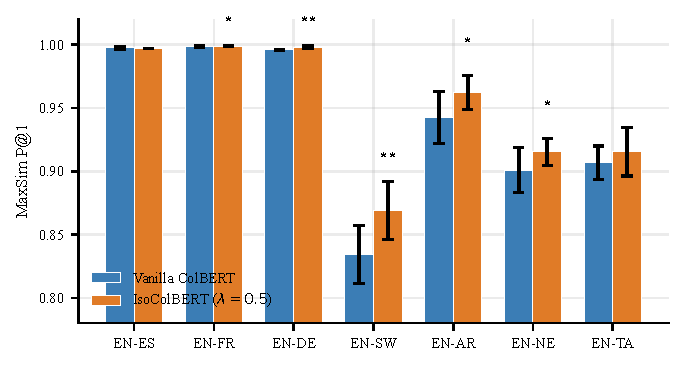
\includegraphics[width=\columnwidth]{figs/fig_main_p1.pdf}
\caption{MaxSim P@1 across seven language pairs, vanilla vs.\ IsoColBERT ($\lambda{=}0.5$), 3-seed mean with $\pm$ standard deviation error bars. Effect-size markers (not statistical significance) compare to vanilla. High-resource pairs are at retrieval ceiling for both methods; the four low-resource pairs (SW, AR, NE, TA) show consistent positive deltas in the mean.}
\label{fig:retrieval}
\end{figure}

\begin{figure}[t]
\centering
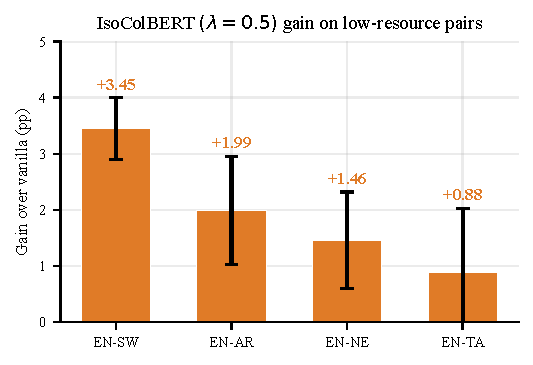
\includegraphics[width=\columnwidth]{figs/fig_low_resource_gains.pdf}
\caption{Pp gain of IsoColBERT over vanilla on the four low-resource pairs (3-seed mean $\pm$ seed-wise std of the gain). The high-resource pairs are saturated in Figure~\ref{fig:retrieval}; this view isolates the regime where the gains live and shows the resource-ordering pattern: the largest gain is on Swahili (lowest pretraining resource), the smallest on Tamil (most pretraining resource among the four).}
\label{fig:retrieval-low}
\end{figure}

\subsection{Retrieval Accuracy}
\label{sec:results-retrieval}

Table~\ref{tab:retrieval} reports MaxSim P@1 across the seven FLORES+ language pairs. On English-Swahili, IsoColBERT improves P@1 from $0.8344 \pm 0.0230$ to $0.8689 \pm 0.0227$, a gain of $3.45$ percentage points; the EN-AR gain is $1.99$ percentage points (from $0.9423$ to $0.9622$). The gains extend zero-shot to Nepali ($+1.46$ pp) and Tamil ($+0.88$ pp), two further low-resource languages that the model never saw during training. The three high-resource pairs (EN-ES, EN-FR, EN-DE) sit at $0.996$ P@1 or above for both methods, with differences within one standard deviation. EN-ES is the only pair on which the model is trained; the other six are evaluated zero-shot, so the low-resource gains transfer through XLM-R's shared multilingual encoder without any in-language supervision. Figure~\ref{fig:retrieval} visualizes the absolute P@1 comparison; Figure~\ref{fig:retrieval-low} zooms in on the four low-resource pairs as pp gain over vanilla, which is where the effect is visible.

\paragraph{Per-seed consistency.} The EN-SW gain is positive on every seed individually: $+3.09$, $+4.08$, and $+3.19$ percentage points on seeds $42$, $1337$, and $2024$ respectively. EN-AR and EN-NE are likewise positive on every seed (EN-AR: $+1.79$, $+1.14$, $+3.04$; EN-NE: $+0.69$, $+1.30$, $+2.39$). EN-TA improves on two of three seeds (with seed $2024$ showing a $-0.45$ pp shift), reflecting the smaller average effect on this pair. The regularizer's seed-wise standard deviation on EN-SW is essentially unchanged from vanilla ($0.0230 \to 0.0227$): the gain is added to a noisy baseline rather than coming from variance reduction.

\paragraph{Where the gains concentrate.} The pattern in Table~\ref{tab:retrieval} is interpretable as the intersection of two conditions: pretrained-signal scarcity and retrieval headroom. High-resource pairs sit at the ceiling because XLM-R was pretrained on far more Spanish, French, and German text than any of the low-resource four, leaving no room for either method to improve. The four low-resource pairs all have weak pretrained signal and room to grow on retrieval, and the largest gain is on the lowest-resource language. Swahili (roughly $1.6$\,GB of pretraining text per \citet{conneau2020xlmr}) sits at the bottom and shows the largest gain ($+3.45$ pp); Arabic ($+1.99$ pp), Nepali ($+1.46$ pp), and Tamil ($+0.88$ pp) follow. The ordering of the latter three is not strictly monotonic in XLM-R pretraining-data size --- Arabic has substantially more pretraining text ($\approx 28$\,GB) than Nepali ($\approx 2.4$\,GB) or Tamil ($\approx 12$\,GB) but a larger gain. Pretrained-signal scarcity is therefore one factor driving the gain pattern, but per-language properties such as script and morphology likely also shape the available retrieval headroom.

\subsection{Token Geometry}
\label{sec:results-geometry}

Table~\ref{tab:geometry} and Figure~\ref{fig:geometry} report the intra-cosine similarity and effective rank of token vectors before and after applying IsoColBERT, for English and Spanish tokens drawn from the FLORES+ dev set. Both metrics move in the direction the regularizer was designed to push them. Intra-cosine drops from $0.20$ to $0.17$ on English and from $0.29$ to $0.18$ on Spanish. Effective rank rises from $105.1$ to $107.5$ on English and from $101.7$ to $106.7$ on Spanish. All four geometric shifts have $\Delta\mu > 2\sigma$ relative to the IsoColBERT seed-wise standard deviation and are consistent in sign across all three seeds.

\begin{table}[t]
\centering
\caption{Token-level geometry on FLORES+ valid token vectors. Intra-cosine is mean off-diagonal cosine over 2048 tokens per language (lower is more isotropic). Effective rank is computed over 4096 tokens per language (higher is more isotropic). Numbers are 3-seed means.}
\label{tab:geometry}
\small
\begin{tabular}{lcccc}
\toprule
 & \multicolumn{2}{c}{Intra-cos $\downarrow$} & \multicolumn{2}{c}{eRank $\uparrow$} \\
\cmidrule(lr){2-3} \cmidrule(lr){4-5}
Method & EN & ES & EN & ES \\
\midrule
Vanilla        & $0.2015$ & $0.2937$ & $105.06$ & $101.73$ \\
IsoColBERT     & $\mathbf{0.1718}$ & $\mathbf{0.1808}$ & $\mathbf{107.50}$ & $\mathbf{106.70}$ \\
$\Delta$       & $-0.030$ & $-0.113$ & $+2.44$ & $+4.98$ \\
\bottomrule
\end{tabular}
\end{table}

\begin{figure*}[t]
\centering
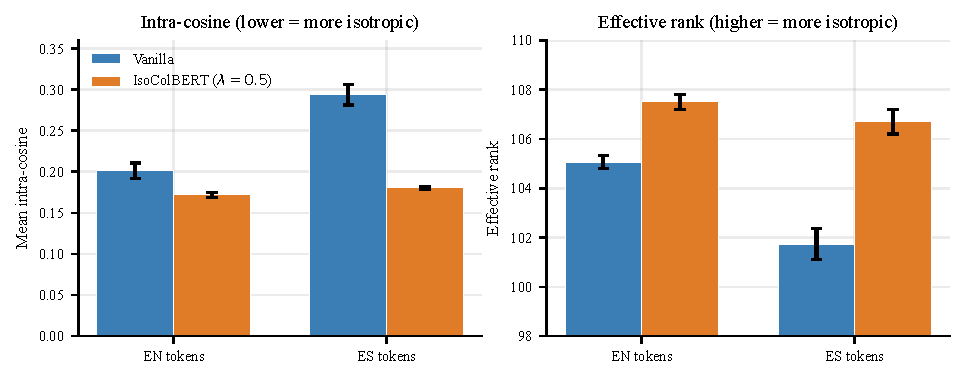
\includegraphics[width=\textwidth]{figs/fig_geometric.pdf}
\caption{Token-level geometry shifts toward isotropy under IsoColBERT. Intra-cosine (left, lower = more isotropic) drops on both languages, with the larger shift on Spanish. Effective rank (right, higher = more isotropic) rises on both languages, again with the larger shift on Spanish. 3-seed mean with $\pm$ standard deviation error bars.}
\label{fig:geometry}
\end{figure*}

\paragraph{Asymmetric collapse and asymmetric recovery.} A consistent pattern across both metrics is that Spanish tokens are more anisotropic than English tokens under vanilla training and more strongly reshaped under IsoColBERT. The vanilla intra-cosine gap is $0.094$ in favor of English ($0.29$ on ES vs.\ $0.20$ on EN); the IsoColBERT gap closes to $0.009$. The effective rank gap closes similarly: $3.33$ down to $0.80$. We attribute the asymmetry to the structure of bitext InfoNCE. The loss in \eqref{eq:infonce} is symmetric in source and target, but the encoder is pretrained on far more English text than Spanish text. Under contrastive pressure, the Spanish-side representations have more to learn and bear most of the gradient signal, which is precisely the regime where the embedding manifold collapses hardest. IsoColBERT redistributes that gradient: instead of letting target-side representations contract into a narrow cone, the regularizer maintains angular separation. This is consistent with the observation that the four low-resource targets — and Swahili in particular — gain the most retrieval accuracy.

\paragraph{Geometry tracks retrieval.} The four geometric metrics (EN/ES intra-cosine, EN/ES effective rank) all clear the \textbf{***} effect-size cutoff ($\Delta\mu > 2\sigma$) with all three seeds positive, and the retrieval gains on the four low-resource pairs (EN-SW, EN-AR, EN-NE, EN-TA) are positive in the mean and on at least two of three seeds in every case. Because the loss in \eqref{eq:loss} explicitly optimizes geometry, this co-movement is correlational rather than causal. We cannot rule out, in particular, that the regularizer also (a) acts as general capacity regularization by penalizing overconfident or high-norm token representations and so improves accuracy through the standard regularization channel; (b) reshapes optimization dynamics indirectly (for example by smoothing the contrastive loss surface) in a way that helps the low-resource pairs disproportionately; or (c) affects cross-lingual alignment through paths that do not pass through token-level intra-cosine and effective rank. What we can say is that geometric reshaping is the only quantity the regularizer directly targets, and that the gain pattern (concentrated on low-resource targets, scaling with vanilla anisotropy) is consistent with the predicted mechanism. Mechanism ablations (Section~\ref{sec:ablations-mechanism}) further constrain the candidates: of the three regularizer placements we tested, only the one that reshapes the full token manifold recovers the retrieval gain.


\section{Ablations}
\label{sec:ablations}

We run two ablations. The first sweeps the regularizer strength $\lambda$ to characterize the trade-off between geometric reshaping and retrieval. The second compares alternative placements of the regularizer to isolate which part of the token manifold is the operative target.

\subsection{Lambda Sweep}
\label{sec:ablations-lambda}

Table~\ref{tab:lambda} reports retrieval and geometry for $\lambda \in \{0, 0.1, 0.5\}$ as three-seed means under the same training protocol used in Section~\ref{sec:results}. Geometry shifts monotonically with $\lambda$. Intra-cosine on Spanish tokens drops from $0.2937$ at $\lambda=0$ to $0.2535$ at $\lambda=0.1$ to $0.1808$ at $\lambda=0.5$. Effective rank on Spanish climbs from $101.7$ to $103.8$ to $106.7$ over the same range. The regularizer continues to reshape the embedding manifold as we increase its weight.

Retrieval P@1 also improves monotonically but with diminishing returns. On EN-SW, the gain is $+3.25$ percentage points from $\lambda=0$ to $\lambda=0.1$, and an additional $+0.20$ percentage points from $\lambda=0.1$ to $\lambda=0.5$. On EN-AR, the gain is $+1.51$ percentage points then $+0.48$ percentage points. We read this as evidence that once anisotropy is no longer the bottleneck, further geometric pressure produces diminishing retrieval gains.

\begin{table}[t]
\centering
\caption{Effect of regularizer strength $\lambda$. Three-seed mean values for EN-SW P@1, EN-AR P@1, intra-cosine on Spanish tokens, and effective rank on Spanish tokens. Geometric metrics improve monotonically; retrieval payoff saturates near $\lambda=0.5$. \textit{Reproducibility note:} the $\lambda=0$ (vanilla) and $\lambda=0.5$ (IsoColBERT) columns are produced by the submitted multi-seed training notebook; the $\lambda=0.1$ column is from a prior 3-seed run conducted under the identical protocol (same architecture, optimizer, batch size, step count, and seed set), included here to characterize the trade-off curve.}
\label{tab:lambda}
\small
\begin{tabular}{lccc}
\toprule
Metric             & Vanilla & $\lambda{=}0.1$ & $\lambda{=}0.5$ \\
\midrule
EN--SW P@1         & $0.8344$ & $0.8669$ & $\mathbf{0.8689}$ \\
EN--AR P@1         & $0.9423$ & $0.9574$ & $\mathbf{0.9622}$ \\
Intra-cos ES $\downarrow$ & $0.2937$ & $0.2535$ & $\mathbf{0.1808}$ \\
eRank ES $\uparrow$       & $101.73$ & $103.78$ & $\mathbf{106.70}$ \\
\bottomrule
\end{tabular}
\end{table}

We select $\lambda = 0.5$ as the headline configuration in Section~\ref{sec:results-retrieval} because it produces the strongest geometric reshaping while remaining within the retrieval-improvement plateau on the low-resource pairs.

\subsection{Mechanism Ablation}
\label{sec:ablations-mechanism}

The uniform regularizer in \eqref{eq:reg} applies pressure to every pair of valid token vectors in the batch. Two natural alternatives restrict the regularization to a subset of tokens or move it from embeddings to matching scores. We compare three placements (each trained with $3$ seeds) to isolate which part of the token manifold is the operative target.

\paragraph{Active-token regularization.} For each query token, MaxSim selects one document token via the argmax in \eqref{eq:maxsim}. The active-token variant regularizes only the query tokens and their selected document tokens, applying \eqref{eq:reg} to the active subset rather than the full token bank.

\paragraph{Cross-attention regularization.} Rather than penalizing redundancy among embedding directions, the cross-attention variant penalizes redundancy among matching patterns. We treat the $L_q \times L_d$ matrix of pairwise similarities as a soft attention map (row-softmaxed across document tokens) and penalize squared off-diagonal correlations between rows. The intuition is to discourage different query tokens from attending to the same document token in similar ways.

\paragraph{Results.} Table~\ref{tab:mechanism} and Figure~\ref{fig:ablation} report the comparison. The uniform regularizer wins on every metric. EN-SW P@1 drops by $2.07$ percentage points under active-token regularization and by $3.68$ percentage points under cross-attention regularization. Intra-cosine on Spanish stays elevated under both alternatives ($0.24$ and $0.30$ vs.\ $0.18$ for uniform). Effective rank on Spanish recovers less ($104.2$ and $101.9$ vs.\ $106.7$).

\begin{table}[t]
\centering
\caption{Mechanism ablation. Three placements of the isotropy regularizer compared on EN-SW retrieval and ES token geometry. Numbers are 3-seed mean $\pm$ std. Uniform (the proposed IsoColBERT objective) strictly outperforms the localized and matching-level alternatives.}
\label{tab:mechanism}
\footnotesize
\setlength{\tabcolsep}{3pt}
\begin{tabular}{lccc}
\toprule
Placement     & EN--SW P@1 & I-cos ES $\downarrow$ & eRank ES $\uparrow$ \\
\midrule
Uniform (ours) & $\mathbf{.869 {\scriptstyle \pm.023}}$ & $\mathbf{.181 {\scriptstyle \pm.002}}$ & $\mathbf{106.7 {\scriptstyle \pm.5}}$ \\
Active-token   & $.848 {\scriptstyle \pm.013}$ & $.239 {\scriptstyle \pm.010}$ & $104.2 {\scriptstyle \pm.8}$ \\
Cross-attn.    & $.832 {\scriptstyle \pm.033}$ & $.299 {\scriptstyle \pm.006}$ & $101.9 {\scriptstyle \pm.2}$ \\
\bottomrule
\end{tabular}
\end{table}

\begin{figure*}[t]
\centering
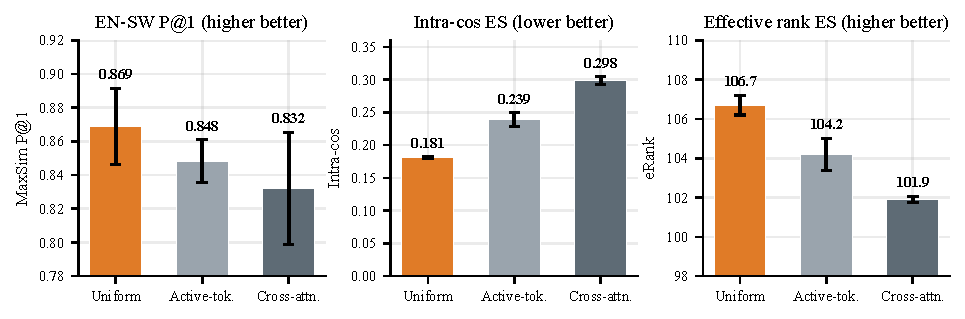
\includegraphics[width=\textwidth]{figs/fig_ablation.pdf}
\caption{Mechanism ablation: regularizing all valid tokens (uniform) outperforms regularizing only MaxSim-winning tokens (active-token) and regularizing the matching score matrix (cross-attention) on EN-SW retrieval and on both geometric metrics. 3-seed mean with $\pm$ standard deviation error bars.}
\label{fig:ablation}
\end{figure*}

\paragraph{Interpreting the localized result.} One reading of why active-token regularization underperforms: it only constrains tokens that already win MaxSim, leaving the losing alternatives unconstrained. If retrieval errors are driven by confusion among the losing tokens, this regularization surface would not directly address them. We caution that this is a post-hoc reading of a single experimental comparison rather than a tested causal mechanism; it is consistent with our results but does not establish that the active-token failure mode is exactly the one described.

\paragraph{Interpreting the object-level result.} A plausible reading of the cross-attention result is that the matching score matrix is a derivative quantity computed from the token vectors, and pushing the rows of the score matrix to be uncorrelated need not make the underlying token vectors more isotropic. Consistent with this reading, the cross-attention variant leaves intra-cosine and effective rank on Spanish near the vanilla baseline ($0.30$ vs.\ vanilla $0.29$; eRank $101.9$ vs.\ vanilla $101.7$) and recovers no retrieval gain. As above, this is a candidate explanation rather than a tested mechanism.

The empirical conclusion we draw from this ablation is narrower than ``broad embedding-space shaping is the mechanism.'' What we can say is that on this benchmark and backbone, of the three placements we tested, only the uniform variant produces both the geometric reshaping and the retrieval gain; the two restricted variants do not substitute for it. Whether other placements (regularizing only document tokens, restricting to a percentile of tokens, or different attention-style targets) could match or exceed uniform regularization remains open.

\section{Discussion and Limitations}
\label{sec:discussion}

\paragraph{What IsoColBERT does and does not do.} The retrieval gains concentrate where two conditions intersect: weak pretrained signal and retrieval headroom. High-resource pairs sit at the P@1 ceiling for both methods, and the small ($-0.05$ pp on EN-ES, not significant) shift on the training pair shows that the regularizer does not damage in-distribution accuracy. The regularizer reshapes geometry in proportion to its weight $\lambda$, but the retrieval payoff saturates once anisotropy stops being the bottleneck. Beyond that point, additional regularization continues to spread the manifold without further accuracy gains.

\paragraph{Asymmetric collapse under bitext contrastive training.} An incidental finding that we have not seen reported elsewhere: under symmetric bitext InfoNCE, the target-side language collapses harder than the source-side language. Spanish tokens have intra-cosine $0.29$ under vanilla training while English tokens have $0.20$; effective ranks are $101.7$ and $105.1$ respectively. We attribute this to the geometry of pretraining: XLM-R is exposed to far more English than Spanish text, so the contrastive objective has more work to do on the Spanish side and the corresponding representations bear most of the gradient pressure. IsoColBERT closes the gap. The geometry of training-pair language asymmetry suggests a diagnostic for predicting which side of a contrastive setup will benefit most from explicit isotropy pressure.

\paragraph{Relation to I-STAR.} \citet{rudman2024istar} report that for classification fine-tuning, decreasing isotropy can improve accuracy. Our result on retrieval is in the opposite direction. The settings differ in two ways that we believe explain the disagreement. First, classification benefits from local clustering: examples of the same class should have nearby representations, which is locally anisotropic. Retrieval benefits from angular separation across the full manifold so that the argmax in MaxSim has high cosine margin. Second, classification operates on sentence-pooled representations, while late-interaction retrieval operates on individual token vectors; the geometric quantity that matters is different. We take this as evidence that the productive direction for isotropy regularization is task-dependent and that retrieval is a clean case where higher isotropy across the embedding manifold is the right objective.

\paragraph{Limitations.} We train on a single language pair (EN-ES) and evaluate transfer to six others. We do not test whether multi-pair training, mixed objectives, or curriculum strategies would further improve the low-resource gains. The backbone is XLM-R base; we do not test whether the effect transfers to larger multilingual encoders or to retrieval-specialized backbones like mE5. The benchmark family is FLORES+; we do not yet test on MIRACL \citep{zhang2023miracl} or mMARCO \citep{bonifacio2021mmarco}, both of which are harder and more realistic retrieval benchmarks. Three seeds is the practical minimum for reporting variance, and we note the per-seed values throughout to allow audit. The $\lambda$ grid is coarse ($\{0, 0.1, 0.5\}$); finer-grained search around $\lambda=0.5$ may yield additional retrieval payoff. Finally, we present mechanism ablations that rule out two alternative regularizer placements, but other placements (for example, regularizing only document tokens, or restricting to a percentile of tokens) remain unexplored.

\section{Conclusion}
\label{sec:conclusion}

We have shown that, in a cross-lingual FLORES+ setup with an XLM-RoBERTa-base backbone, token-level anisotropy is a measurable property of vanilla multilingual ColBERT and one that can be reshaped with a single regularizer term added to InfoNCE training. The regularizer has one hyperparameter and zero inference cost; it improves token-embedding geometry monotonically with regularization strength and recovers $+3.45$ percentage points of MaxSim P@1 on English-Swahili and $+1.99$ percentage points on English-Arabic, with the gains extending zero-shot to two further low-resource languages (Nepali $+1.46$, Tamil $+0.88$). Mechanism ablations against active-token and cross-attention placements show that, of the three placements we tested, the uniform variant is the only one that produces both the geometric reshaping and the retrieval gain. We caution that all of these claims are tied to our specific evaluation setting; whether the same geometric pathology drives retrieval errors on harder benchmarks (MIRACL, mMARCO) or on larger and retrieval-specialized backbones (multilingual E5) remains an empirical question for future work. Within the setting we evaluate, however, token geometry is a tractable lever for low-resource multilingual retrieval.


\bibliography{refs}
\bibliographystyle{icml2026}

\end{document}
